
\documentclass[12]{article}

\usepackage{graphicx}
\usepackage{framed}
\usepackage{listings}
\usepackage{titlesec}
\usepackage{tikz}
\usepackage{amssymb}
\usepackage{amsmath}
\usepackage{MnSymbol}
\newcommand{\sectionbreak}{\clearpage}

\lstset{frame=tb,
  language=Java,
  aboveskip=3mm,
  belowskip=15mm,
  showstringspaces=false,
  columns=flexible,
  basicstyle={\small\ttfamily},
  numbers=none,
  breaklines=true,
  breakatwhitespace=true
  tabsize=3
}


\newtheorem{theorem}{Theorem}[section]
\newtheorem{lemma}[theorem]{Lemma}
\newtheorem{proposition}[theorem]{Proposition}
\newtheorem{corollary}[theorem]{Corollary}

\newenvironment{proof}[1][Proof]{\begin{trivlist}
\item[\hskip \labelsep {\bfseries #1}]}{\end{trivlist}}
\newenvironment{definition}[1][Definition]{\begin{trivlist}
\item[\hskip \labelsep {\bfseries #1}]}{\end{trivlist}}
\newenvironment{example}[1][Example]{\begin{trivlist}
\item[\hskip \labelsep {\bfseries #1}]}{\end{trivlist}}
\newenvironment{remark}[1][Remark]{\begin{trivlist}
\item[\hskip \labelsep {\bfseries #1}]}{\end{trivlist}}



\newcommand{\qed}{\nobreak \ifvmode \relax \else
      \ifdim\lastskip<1.5em \hskip-\lastskip
      \hskip1.5em plus0em minus0.5em \fi \nobreak
      \vrule height0.75em width0.5em depth0.25em\fi}
\newcommand{\pre}{\mathop{\mathrm{pre}}}
\newcommand{\myparagraph}[1]{\paragraph{#1}\mbox{}\\}



\begin{document}

\tableofcontents
\section*{Abstract}

\section{Introduction}

\subsection{The Problem}

We are becoming increasingly dependent on computer systems. Not only are they an essential part of our lives, ...vital!



\subsection{The Idea}

\subsection{The Deliverables}


\begin{itemize}
\item Autonomous systems, what they are, why they are useful, and why they are vulnerable but we need to make sure they are reliable.
\item Verifying autonomous systems: what it entails, how we go about it (methods) and what are the challenges
\item The state explosion problem
\item Our idea and contributions
\item structure of the report
\end{itemize}

\section{Background}

\subsection{Logics for Multi-Agent Systems}

\subsubsection{Multi-Agent Systems}

Autonomous multi-agent systems are computer systems which are made up of several intelligent ``agents" acting within an ``environment". 
Intuitively, an \textit{agent} is: 
\begin{itemize}
\item Capable of \textit{autonomous} action 
\item Capable of \textit{social} interaction with its peers
\item Acting to \textit{meet} their design objectives 
\end{itemize}
 
Suppose we have a multi-agent systems consisting of $n$ agents and an environment $e$.
\begin{definition} 
An agent $i$ in the system consists of: 
\begin{itemize}
\item A set $L_i$ of local states representing the different configurations of the agent,
\item A set $Act_i$ of local actions that the agent can take,
\item A protocol function $P_i : L_i \rightarrow 2^{Act_i} $ expressing the decision making of the agent.
\end{itemize} 
\end{definition}

We can define the environment $e$ as a similar structure $(L_e, Act_e, P_e)$ where $P_e$ represents the functioning conditions of the environment. 

\subsubsection{Interpreted Systems}
\label{IS}
We present a formal structure to represent multi-agent systems. Consider a multi-agent system $\Sigma$ consisting of $n$ agents $1, ..., n$ and an environment $e$.
\begin{definition}
An \textit{Interpreted System} $IS$ for $\Sigma$ is a tuple $(G, \tau, I, \sim_1, ..., \sim_n, \pi)$, where
\begin{itemize}
\item $G \subseteq L_1 \times ... \times L_n \times L_e$ is the set of global states that $\Sigma$ can reach. A global state $g \in G$ is essentially a picture of the system at a given point in time, and the local state of agent $i$ in $g$ is denoted $l_i(g)$.
\item $I \subseteq G$ is a set of intial states for the system
\item $\tau : G \times Act \rightarrow G $ where $Act = Act_1 \times ... \times Act_n \times Act_e$ is a deterministic transition function (we can define $\tau : G \times Act \rightarrow 2^G$ to model a non-deterministic system)
\item $\sim_1, ..., \sim_n \subseteq G \times G$  are binary relations defined by $$g \sim_i g' \Leftrightarrow l_i(g) = l_i(g') \quad \forall g, g' \in G, \forall i = 1, ..., n$$
i.e iff agent $i$ is in the same state in both $g$ and $g'$. 
\item $\pi : PV \rightarrow G$ is a valuation function for the set of atoms $PV$, i.e for each atom $p \in PV$, $\pi(p)$ is the set of global states where $p$ is true
\end{itemize}
\end{definition}

We also need a formal definition for the ``execution'' of a system. A \emph{run}, as defined below, represents one possible execution of a MAS. 
\begin{definition} 
A \emph{run} of an interpreted system $IS = (G, \tau, I, \sim_1, ..., \sim_n, \pi)$ is a sequence $r = g_0, g_1, ...$ where $g_0 \in I$ and such that for all $i \geq 0$, $\exists a \in Act$ such that $\tau(g_i, a) = g_{i+1}$.
\end{definition}

Interpreted Systems as defined above are used as semantic structures for a particular family of logics, presented in the next section.

\subsubsection{Linear Temporal Logic} 
\label{LTL}

In order to verify properties of multi-agent systems, we first need to find a logic allowing us to describe these properties accurately. 

A good candidate is the Linear Temporal Logic (LTL), a modal temporal logic in which one can write formulas about the future of \emph{paths}. Here we use paths to represent infinite runs of an interpreted system. 

\begin{definition} 
The syntax of LTL formulas is given by the following BNF: 
$$\varphi := p \mid \lnot\varphi \mid \varphi \land \varphi \mid X\varphi \mid G\varphi \mid \varphi U\varphi$$
\end{definition}

The intuitive meanings of $X\varphi, G\varphi$ and $\varphi U\psi$ are respectively 
\begin{itemize} 
\item $\varphi$ holds at the ne\textbf{X}t time instant
\item $\varphi$ holds forever (\textbf{G}lobally)
\item $\varphi$ holds \textbf{U}ntil $\psi$ holds  
\end{itemize}

We define the unary operator $F$ to be the dual of $G$, i.e $F\varphi := \lnot G\lnot\varphi$ for any LTL formula $\varphi$. $F\varphi$ represents the idea that $\varphi$ will hold at some point in the \textbf{F}uture.   

\myparagraph{Semantics} 

A model for LTL is a Kripke model $M = (W, R, \pi)$ such that the relation $R$ is serial, i.e $\forall u \in W,  \exists v \in W$ such that $(u, v) \in R$.
The worlds in $W$ are called the \textit{states} of the model. 

\begin{definition} 
A \textit{path} in an LTL model $M = (W, R, \pi)$ is an infinite sequence of states $\rho = s_0, s_1, ...$ such that $(s_i, s_{i+1}) \in R$ for any $i \geq 0$.
We denote $\rho^i$ the suffix of $\rho$ starting at $i$ (note that $\rho^i$ is itself a path since $\rho$ is infinite).
\end{definition}

It is easy to see how such a model can be used to represent a computer system, and how an execution of this system can be written as a path.

 Our objective is to be able to verify that a system $S$ has property $P$, so if we encode $P$ as an LTL formula $\varphi_P$ and $S$ as a model $M_S$, then we need to be able to check whether $\varphi_P$ is \textit{valid} in $M$ (or at least true in a set of initial states). This technique is called \textit{model checking}, and we do this by using the following definition for the semantics of LTL:
\label{model_checking}

\begin{definition}
Given LTL formulae $\varphi$ and $\psi$, a model $M$ and a state $s_0 \in W$, we say that
\begin{eqnarray*}
(M, s_0) \models p &\Leftrightarrow& s_0 \in \pi(p) \\  
(M, s_0) \models \lnot \varphi &\Leftrightarrow& (M, s_0) \nmodels \lnot \varphi\\
(M, s_0) \models \varphi \land \psi &\Leftrightarrow& (M, s_0) \models \varphi \mbox{ and  } (M, s_0) \models \psi \\
(M, s_0) \models X\varphi &\Leftrightarrow& (M, s_1) \models \varphi \mbox{  for all states } s_1 \mbox{ such that } R(s_0, s_1)\\
(M, s_0) \models G\varphi &\Leftrightarrow& \mbox{for all paths } \rho = s_0, s_1, s_2, ... , \mbox{ we have } (M, s_i) \models \varphi \quad \forall i \geq 0 \\
(M, s_0) \models \varphi U\psi &\Leftrightarrow& \mbox{for all paths } \rho = s_0, s_1, s_2, ..., \exists j \geq 0 \mbox{ such that }  (M, s_j) \models \psi \\ && \mbox{ and }  (M, s_k) \models \varphi \quad \forall 0 \leq k < j
\end{eqnarray*}

\end{definition}

The expressive power of LTL is limited to quantification over \textit{all} possible paths. For example: 

\begin{itemize}
\item $FG($deadlocked$)$ 

In every possible execution, the system will be permanently deadlocked.

\item $GF($crash$)$

Whatever happens, the system will crash infinitely often.
\end{itemize}

Hence some properties cannot be expressed in LTL, as in certain applications we might want to quantify explicitely over paths. The Computation Tree Logic (CTL) can express this. 

\subsubsection{Computation Tree Logic} 

\begin{definition} 
The syntax of CTL formulae is defined as follows: 
$$ \varphi := p \mid \lnot \varphi \mid \varphi \land \varphi \mid EX\varphi \mid EG\varphi \mid E(\varphi U \varphi)$$
\end{definition}

Intuitively, $ EX\varphi,  EG\varphi,$ and $ E(\varphi U \psi)$ represent the fact that there exists a possible path starting from the current state such that, respectively, $\varphi$ is true at the next state, $\varphi$ holds forever in the future, and $\varphi$ holds until $\psi$ becomes true.

The dual operator $AX\varphi := \lnot EX \lnot\varphi $ can be used to represent the fact that in all possible paths from the current state, $\varphi$ is true at the next state.
Connectives $AG\varphi, AF\varphi,$ and $A(\varphi U\psi)$ can be defined in the same way. 

We also use models (as defined in \ref{LTL}) for the semantics of CTL, as follows:

\begin{definition} 
Given CTL formulas $\varphi$ and $\psi$, a model $M = (W, R, \pi)$ and a state $s_0 \in W$, the satisfaction of formulas at $s_0$ in $M$ is defined inductively as follows: 
\begin{eqnarray*}
(M, s_0) \models p &\Leftrightarrow& s_0 \in \pi(p) \\  
(M, s_0) \models \lnot \varphi &\Leftrightarrow& (M, s_0) \nmodels \lnot \varphi\\
(M, s_0) \models \varphi \land \psi &\Leftrightarrow& (M, s_0) \models \varphi \mbox{ and  } (M, s_0) \models \psi \\
(M, s_0) \models EX\varphi &\Leftrightarrow& \exists \mbox{ a path } s_0, s_1, s_2, ... \mbox{ such that } (M, s_1) \models \varphi \\
(M, s_0) \models EG\varphi &\Leftrightarrow& \exists \mbox{ a path } s_0, s_1, s_2, ... \mbox{ such that } (M, s_i) \models \varphi \quad \forall i \geq 0\\
(M, s_0) \models E(\varphi U\psi) &\Leftrightarrow&  \exists \mbox{ a path } s_0, s_1, s_2, ... \mbox{ for which } \exists i \geq 0 \mbox{ such that }  (M, s_i) \models \psi \\ && \mbox{ and }  (M, s_j) \models \varphi \quad \forall 0 \leq j < i
\end{eqnarray*}
\end{definition}

The quantifiers allow for more properties to be expressed, for example:
\begin{itemize}
\item From any state it is possible to reboot the system.

$AGEX($reboot$)$ \quad (not expressible in LTL)

\item example 2


\end{itemize}

Again, some formulas can be expressed in LTL but not in CTL. For instance, the property that \textit{in every path where $p$ is true at some point then $q$ is also true at some point} is expressed in LTL as $Fp \rightarrow Fq $ but there is no equivalent CTL formula.
 The logic CTL* combines the syntax of LTL and CTL to provide a richer set of connectives. We will not go into any more details regarding CTL*, but we refer the reader to TODO for more information. 

\subsubsection{The Epistemic Logic CTLK}

In the case of multi-agent systems, we are interested in describing the system in terms of individual agents, and in particular their \textit{knowledge}. 

For this reason, we add a family of unary operators $K_i$ for $i = 1, ..., n$ to the modal connectives defined previously. Each $K_i$ will represent the intuitive notion of knowledge for agent $i$. 
This enables us to define the temporal-epistemic logics LTLK and CTLK, which are extensions of LTL and CTL, respectively. Here we leave out details about LTLK, as the practical applications we present later on only support CTLK. 



\begin{definition} 
The syntax of CTLK is defined by the following BNF: 
$$ \varphi := p \mid \lnot \varphi \mid \varphi \land \varphi \mid EX\varphi \mid EG\varphi \mid E(\varphi U \varphi) \mid  K_i\varphi \quad (i \in \{1, ..., n\})$$
\end{definition}  

We use interpreted systems (\ref{IS}) as semantic structures for CTLK. The satisfaction of a CTL formula on an interpreted system $IS$ is defined analogously to its satisfaction on a model $M$ whose worlds $W$ are the global states of $IS$, and whose relation function $R$ is the global transition function of $IS$. 
For example, $(IS, g_0) \models EX\varphi \mbox{  iff there is a run } r = g_0, g_1, g_2, ... \mbox{ of $IS$ such that } (IS, g_1) \models \varphi$.

The following definition completes the semantics of CTLK formulae:

\begin{definition}
Given an interpreted system $IS$, a global state $g$, an agent $i$ of $IS$, and a CTLK formula $\varphi$, we define
$$(IS, g) \models K_i \varphi \mbox{  iff  } \forall g' \in G, g \sim_i g' \Rightarrow (IS, g') \models \varphi$$

The connective $K_i$ expresses that agent $i$ \emph{knows} of the property $\varphi$ when the system's global state is $g$.

We extend the syntax and semantics of CTLK by adding two extra unary operators: $E$ (Everybody knows) and $C$ (Common knowledge), whose semantics are defined as follows:

\begin{eqnarray*}
(IS, g_0) \models E\varphi &\Leftrightarrow& (IS, g_0) \models K_i \varphi \quad \forall i = 1, ..., n \\
(IS, g_0) \models C\varphi &\Leftrightarrow&  (IS, g_0) \models \bigwedge^\infty_{k = 1} E^{(k)}\varphi \quad \\&& \mbox{ where } E^{(1)} = E \mbox{ and } E^{(j+1)} = EE^{(j)} \quad \forall j \geq 1
\end{eqnarray*}
\end{definition}


\subsection{Model Checking}

Model checking was briefly introduced in \ref{model_checking} as a automated verification technique, which can be used to check that a system $S$ satisfies a specification $P$. The technique involves representing $S$ as a logic system $L_S$ which captures all possible computations of $S$, and encoding the property $P$ as a temporal formula $\varphi_P$. 

The problem of verifying $P$ is then reduced to the problem of checking whether $L_S \vdash \varphi_P $. But we can now build a Kripke model $M_S = (W_S, R_S, \pi)$ such that $L_S$ is sound and complete over (the class of) $M_S$, so that $$L_S \vdash \varphi_P \Leftrightarrow M_S \models \varphi_P .$$ 
$M_S$ is the Kripke model representing all possible computations of $S$, i.e. $W_S$ contains all the possible computational states of the system and the relation $R_S$ represents all temporal transitions in the system. 

In the case of a multi-agent system as defined above, encoding $S$ as an interpreted systems of agents will satisfy the equivalence. 

\subsubsection{Explicit Model Checking}

\label{explicit}
In this section we introduce a basic approach to model checking, the so-called \textit{explicit} approach.

Suppose that we want to check that a multi-agent system $\Sigma$ satisfies a propery $P$. If $IS$ is an interpreted system representing $\Sigma$, and $\varphi$ the CTLK formula corresponding to $P$, we need to verify that $(IS, s_0) \models \varphi$, for all initial states $s_0 \in I$.

Algorithmically it is more efficient \cite{need ref} to compute the set of global states $[\varphi]$ of $IS$ where $\varphi$ is true, and check that $I \subseteq [\varphi]$. 
The following algorithm returns $[\varphi]$ for any CTLK formula $\varphi$.


\begin{lstlisting}[mathescape]

function SAT($\varphi$) 
// returns $[\varphi]$
if $\varphi = \top$: return $G$
if $\varphi = \bot$: return $\varnothing$
if $\varphi = p$: return $\pi(p)$ 
if $\varphi = \lnot\varphi_1$: return $G \setminus$SAT($\varphi_1$)
if $\varphi = \varphi_1\land\varphi_2$: return SAT($\varphi_1$)$\cap$SAT($\varphi_2$)
if $\varphi = EX\varphi_1$: return SAT$_{\mbox{EX}}(\varphi_1)$
if $\varphi = AF\varphi_1$: return SAT$_{\mbox{AF}}(\varphi_1)$
if $\varphi = E(\varphi_1 U\varphi_2 )$: return SAT$_{\mbox{EU}}(\varphi_1, \varphi_2)$
if $\varphi = K_i\varphi_1$: return SAT$_{\mbox{K}}(i, \varphi_1)$
if $\varphi = E\varphi_1$: return SAT$_{\mbox{E}}(\varphi_1)$
if $\varphi = C\varphi_1$: return SAT$_{\mbox{C}}(\varphi_1)$
end
$\\$
\end{lstlisting}

Notice that this covers all formulae $\varphi$, as $\{EX, AF, EU, K_i, E, C\}$ is a minimum set of connectives for CTLK. The respective auxilliary functions are defined below. Notation: for any global states $g_0, g_1$ of $IS$ we write $g_0 \rightarrow g_1$ iff $\exists a \in Act$ such that $\tau(g_0, a) = g_1$ (i.e. there is an run of $IS$ starting with $g_0, g_1, ...$).


\begin{lstlisting}[mathescape]

function SAT$_{\mbox{EX}}$($\varphi$)
// returns $[EX\varphi]$
  X := {$g_0 \in G \mid g_0 \rightarrow g_1$ for some $g_1 \in $SAT($\varphi$) }
  return X
end
 
function SAT$_{\mbox{AF}}$($\varphi$)
// returns $[AF\varphi]$
  X := $G$
  Y := SAT($\varphi$)
  repeat until X = Y:
    X := Y
    Y := Y $\cup$ $\{ g_0 \in G \mid $ for all $g_1 $ with $g_0 \rightarrow g_1$, $g_1 \in$ Y $\}$ 
  end
  return Y
end
  

function SAT$_{\mbox{EU}}$($\varphi_1$, $\varphi_2$)
// returns $[E(\varphi_1U\varphi_2)]$
  W := SAT($\varphi$)
  X := $G$
  Y := SAT($\psi$)
  repeat until X = Y:
    X := Y
    Y := Y $\cup$ (W $\cap$ $\{g_0 \in G \mid \exists g_1 \in$ Y such that $g_0 \rightarrow g_1\}$)
  end
  return Y
end

function SAT$_{\mbox{K}}$($i$, $\varphi$)
// returns $[K_i\varphi]$
  X := SAT($\lnot\varphi$)
  Y := $\{g_0 \in G \mid \exists g_1 \in$ X with $R_i(g_0, g_1)\}$
  return $G \setminus\mbox{Y}$
end

function SAT$_{\mbox{E}}$($\varphi$)
// returns $[E\varphi]$
  X := SAT($\lnot\varphi$)
  Y := $\{g_0 \in G \mid \exists g_1 \in$ X with $R_i(g_0, g_1)$ for all $i = 1, ..., n\}$
  return $G \setminus\mbox{Y}$
end

function SAT$_{\mbox{C}}$($\varphi$)
// returns $[C\varphi]$
  X := $G$
  Y := SAT($\lnot\varphi$)
  repeat until X = Y:
    X := Y
    Y := $\{g_0 \in G \mid \exists g_1 \in$ X with $R_i(g_0, g_1)$ for all $i = 1, ..., n\}$
  end
  return $G \setminus\mbox{Y}$
end

\end{lstlisting}

TODO write something about $R_i$. 

The complexity of \texttt{SAT} is linear in the size of the model. However, the size of the model grows exponentially in the number of variables used to describe the system $\Sigma$, therefore the explicit approach is not always viable in practice. This is the main difficulty in model checking and it is known as the \textit{state explosion problem}. 

In the next section we introduce a model checking technique aiming to improve the efficiency of the approach. 

\subsubsection{Symbolic Model Checking}

\textit{Symbolic model checking} is an approach to model checking which involves representing sets of states and functions between them as Boolean formulas. The algorithm presented in \ref{explicit} is then reduced to a series of operations on Boolean formulas. In this section we go through the process of encoding sets and functions as propositional formulas, and we explain how this encoding facilitates model checking.

\myparagraph{Symbolic Representation of Sets of States}
\label{symbolic}
\begin{figure}
    \centering
    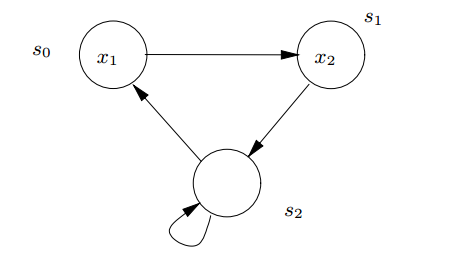
\includegraphics[scale=0.55]{symbolic_model_checking_example.PNG}
    \caption{A model}
    \label{fig:model_example}
\end{figure}

The encoding process is best illustrated by an example  \cite{logic_in_computer_science}
Consider the model in Figure~\ref {fig:model_example}, representing a system with three states labelled $s_0, s_1, s_2$. 

We consider two propositional variables, namely $x_1$ and $x_2$.  
If $S$ is the whole state space (so $S = \{s_0, s_1, s_2\}$), we can represent subsets of $S$ using Boolean formulae, as shown in the following table:\\

\begin{tabular}{ l | r }
  set of states & representation by boolean formula \\ \hline
$\emptyset $&   $\bot$ \\
$\{ s_0\}$ & $x_1 \land \lnot x_2 $\\
$\{ s_1\}$ & $ \lnot x_1 \land x_2 $\\
$\{ s_2\}$ & $\lnot x_1 \land \lnot x_2 $\\
$\{ s_0, s_ 1\}$ & $(x_1 \land \lnot x_2) \lor (\lnot x_1 \land x_2)  $\\
$\{ s_1, s_2\}$ & $(\lnot x_1 \land  x_2) \lor (\lnot x_1 \land\lnot x_2)$\\
$\{ s_0, s_2\}$ & $(x_1 \land \lnot x_2) \lor (\lnot x_1 \land\lnot x_2) $\\
$\{ s_0, s_1, s_2\}$ & $(x_1 \land \lnot x_2) \lor (\lnot x_1 \land  x_2) \lor (\lnot x_1 \land\lnot x_2)$
\end{tabular}
\\
\\

Note that for this representation to be unambiguous, we must ensure that no two states satisfy the same set of Boolean variables. If this is the case, new variables can be added which will be used to differenciate between the ambiguous states.

\myparagraph{Symbolic Representation of a Transition Relation}

The transition relation $\rightarrow$ of a model is a subset of $S \times S$. Taking two copies of our set of propositional variables, we can then associate a Boolean formula to the transition relation. In the example above, the transition relation $\rightarrow$ of the model is $\{(s_0, s_1), (s_1, s_2), (s_2, s_0), (s_2, s_2)\}$. 
Using our Boolean representations for $s_0, s_1$, and $s_2$, we compute the representation of $\rightarrow$ to be $$(\lnot x_1 \land \lnot x_2 \land \lnot x'_1 \land \lnot x'_2 ) \lor (\lnot x_1 \land \lnot x_2 \land x'_1 \land \lnot x'_2 ) \lor ( x_1 \land \lnot x_2 \land \lnot x'_1 \land  x'_2 ) \lor (\lnot x_1 \land x_2 \land \lnot x'_1 \land \lnot x'_2 )$$

[needs more details on the computation]\\\\

\myparagraph{The case of Multi-Agent Systems}

need to explain this

How does this help us? Well, several techniques exist which allow us to represent these Boolean formulas in a very concise form. This is the topic of the next section.

\subsection{Representing Boolean functions}

It is important to make the point that the Boolean formulas computed in \ref{symbolic} can be regarded as Boolean \textit{functions}, i.e. functions $\{0, 1\}^n \rightarrow \{0, 1\}$ for some $n$. For example, the formula $x_1 \land \lnot x_2$ is associated to the function $f(x_1, x_2) = x_1 \land \lnot x_2$.

In this section we introduce a theory of representations of Boolean functions using directed acyclic graphs (DAG). 

\subsubsection{Ordered Binary Decision Diagrams}

After truth tables, one the most basic ways of representing Boolean functions is by using a \textit{binary decision tree} (BDT). A BDT is a binary tree where we label non-terminal nodes with Boolean variables $x_1, x_2, ...$ and terminal nodes with the values 0 and 1. Each non-terminal node has two outgoing edges, one solid and one dashed (one for each value of the variable the node is labelled with). An example is shown in Figure~\ref{fig:BDT}. Note that the initial ordering of the variables changes the resulting BDT; for convenience, we write $[x_1, x_2, ..., x_n]$ to denote the order $x_1 < x_2 < ... < x_n$.


BDTs are a relatively inefficient way of storing Boolean formulas, since a BDT for a formula with $n$ variables will have $2^{n+1} - 1$ nodes. Fortunately, a BDT can be reduced to an \textit{ordered binary decision diagram} (OBDD), a much more compact data structure.

\begin{figure}
\centering
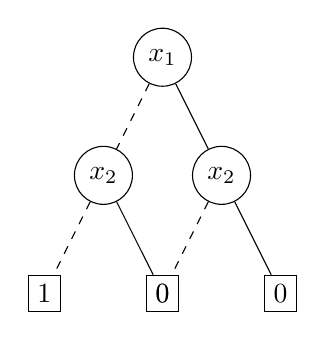
\begin{tikzpicture}

	[level 1/.style={sibling distance=33mm},
	 level 2/.style={sibling distance=23mm}]
	\node[circle, draw] (x1) {$x_1$}	 
		child {node[circle,draw] (x21) {$x_2$} [dashed]
			child {node[rectangle, solid, draw] (1) {1} [dashed]}
			child {node[rectangle, solid, draw] (01) {0} [solid]}}
		child {node[circle,draw] (x22) {$x_2$} [solid]
			child {node[rectangle, solid, draw] (02) {0} [dashed]}
			child {node[rectangle, solid, draw] (03) {0} [solid]}};
\end{tikzpicture}
	\caption{BDT for $f(x_1, x_2) = x_1 \land \lnot x_2$ under the ordering $[x_1, x_2]$}
\label{fig:BDT}
\end{figure}

\myparagraph{The Reduction Algorithm} 

There are three steps in the reduction of BDTs to OBDDs:
\begin{enumerate}
\item Removal of duplicate terminals: we merge all the 0-nodes and 1-nodes into two unique terminal nodes
\item Removal of redundant tests: if both outgoing edges of a node $n$ point to the same node $m$, we remove $n$ from the graph, sending all its incoming edges directly to $m$ 
\item Removal of duplicate non-terminals: we merge any two subtrees with identical BDD structure
\end{enumerate}

Steps (2) and (3) are repeatedly applied until no further reduction is possible. The resulting diagram is said to be a ordered binary decision diagram. 

[here need example of using reduction algorithm]

The following key result makes the use of OBDDs viable in practice: 

\begin{theorem}
\label{obdd_uniqueness}
If $f$ is a Boolean function over the variables $x_1, ..., x_n$, then the OBDD representing $f$ is unique, up to the order of $x_1, ..., x_n$ chosen.
\end{theorem}

The immediate consequence of Theorem~\ref{obdd_uniqueness} is that one can easily compare two Boolean functions by comparing their respective OBDDs (provided both OBDDs have the same variable order). 

Another important observation to make is that OBDDs resulting from two different variable orders may present a \textit{significant }difference in size, and therefore a large amount of work has been done in the search for suitable variable orders. 

OBDDs help us to manipulate Boolean functions with a high number of variables, allowing us to use our model checking algorithm (\ref{explicit}) on systems with much larger state-spaces, which has led researchers in the past 15 years to explore various graph-based representations of Boolean functions.

\noindent\textit{Note to the reader: throughout this report we often drop the `O' and refer to OBDDs as BDDs.}

\subsubsection{A Knowledge Compilation Map}

In computer science, the field of \textit{knowledge compilation} is concerned with finding compact and efficient representations of propositional knowledge bases (such as symbolic representations of state-spaces, cf \ref{symbolic}).
 Such a representation is refered to as a \textit{target compilation language}, of which BDTs and OBDDs are examples. 
 
 The main properties that we look for in a target compilation language are the canonicity of the representation, the succinctness of the representation, and a polynomial-time complexity for queries and operations on the language. 
 These properties will ensure that we can safely rely on a particular language for our model checking algorithm. 
 
 OBDDs satisfy these properties (with succintness remaining highly dependent on the variable order), and in fact a number of model checkers use them for state-space representation (e.g. NuSMV, MCMAS). 
 
 In 2002, A. Darwiche and P. Marquis published \cite{compilation_map} a comparative analysis of most existing DAG-based target compilation languages in terms of their succintness and the polytime operations they support. They show that all of these languages are subsets of a broad language called \textit{negation normal form} (NNF). 

\begin{definition}
A sentence in \textit{NNF} is a rooted directed acyclic graph where each leaf node is labelled with $\top$, $\bot$, $X$ or $\lnot X$ for some propositional variable $X$, and each internal node is labelled with $\land$ or $\lor$ and can have arbitrarily many children. 

\end{definition} 

\noindent Remark: OBDDs are NNF sentences. Figure~\ref{nnf_obdd} shows an OBDD and its corresponding NNF sentence.  

\begin{figure}
\centering
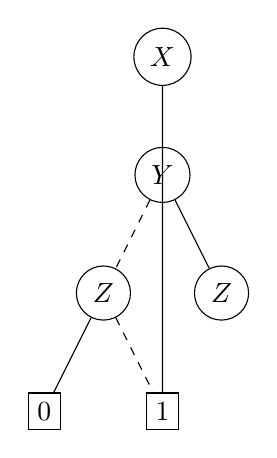
\begin{tikzpicture}

	[level 1/.style={sibling distance=33mm},
	 level 2/.style={sibling distance=23mm},
	 level 3/.style={sibling distance=16mm}]
	\node[circle, draw] (X) {$X$}	 
		child {node[circle, solid, draw] (Y) {$Y$} [dashed]
			child {node[circle, solid, draw] (Z1) {$Z$} [dashed]
				child {node[rectangle, solid, draw] (0) {0} [solid]}
				child {node[rectangle, solid, draw] (1) {1} [dashed]}}
			child {node[circle, solid, draw] (Z2) {$Z$} [solid]}};
	\draw[solid] (X) -- (1); 
\end{tikzpicture}
\qquad\quad
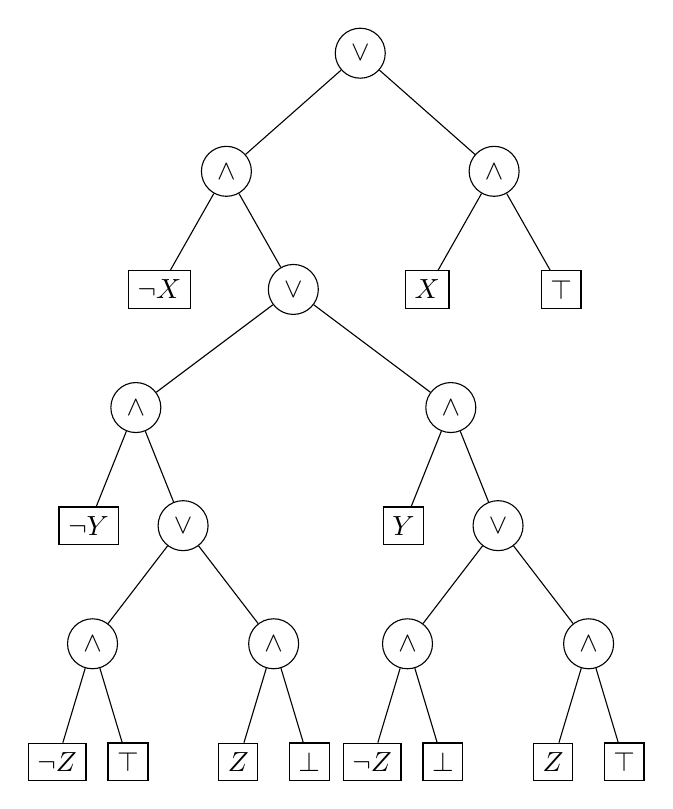
\begin{tikzpicture}
	[level 1/.style={sibling distance=34mm},
	 level 2/.style={sibling distance=17mm},
	 level 3/.style={sibling distance=40mm},
	 level 4/.style={sibling distance=12mm},
	 level 5/.style={sibling distance=23mm},
	 level 6/.style={sibling distance=9mm}]
	\node[circle, draw] (or1) {$\lor$}	 
		child {node[circle,draw] (and1) {$\land$} [solid]
			child {node[rectangle, solid, draw] (X1) {$\lnot X$}[solid]}
			child {node[circle, solid, draw] (or2) {$\lor$} [solid]
				child {node[circle,draw] (and3) {$\land$} [solid]
					child {node[rectangle, solid, draw] (Y1) {$\lnot Y$}[solid]}
					child {node[circle, solid, draw] (or5) {$\lor$} [solid]
						child {node[circle,draw] (and5) {$\land$} [solid]
							child {node[rectangle, solid, draw] (Z1) {$\lnot Z$}[solid]}
							child {node[rectangle, solid, draw] (T2) {$\top$} [solid]} 	
						}
						child {node[circle,draw] (and6) {$\land$} [solid]
							child {node[rectangle, solid, draw] (Z2) {$Z$}[solid]}
							child {node[rectangle, solid, draw] (F1) {$\bot$} [solid]} 	
						}
					}
				}
				child {node[circle,draw] (and4) {$\land$} [solid]
					child {node[rectangle, solid, draw] (Y2) {$Y$}[solid]}
					child {node[circle, solid, draw] (or6) {$\lor$} [solid]
						child {node[circle,draw] (and7) {$\land$} [solid]
							child {node[rectangle, solid, draw] (Z3) {$\lnot Z$}[solid]}
							child {node[rectangle, solid, draw] (F2) {$\bot$} [solid]} 	
						}
						child {node[circle,draw] (and8) {$\land$} [solid]
							child {node[rectangle, solid, draw] (Z2) {$Z$}[solid]}
							child {node[rectangle, solid, draw] (T2) {$\top$} [solid]} 	
						}
					}
				}
			}
		}
		child {node[circle,draw] (and2) {$\land$} [solid]
			child {node[rectangle, solid, draw] (X2) {$X$} [solid]}
			child {node[rectangle, solid, draw] (T1) {$\top$} [solid]}
		};
\end{tikzpicture}

	\caption{An OBDD (left) and its corresponding NNF sentence (right). Although the former seems much more compact, the difference in size is only linear and both representations are essentially the same. TODO sort this oout}
\label{nnf_obdd}

\end{figure}
 
 
 
\subsubsection{Project Directions}

 This ``knowledge compilation map" was the starting point for this project, whose initial objective was to investigate new target compilation languages suitable for application to model checking, seeking a potential improvement on BDDs (which constitute so far the ``industry standard").

 Taking into account the various criteria for suitable representations described above, we searched the literature aiming to find a good candidate to replace BDDs. 

After considering a number of different representations including tree-of-BDDs \cite{trees_of_bdds}, BDD-trees \cite{bdd_trees}, and several other subsets of NNF described in \cite{compilation_map}, we opted for a relatively novel target compilation language called \textit{sentential decision diagram} (SDD). 

SDDs are a subset of NNF, possess the required properties, and had not yet been experimented with in the context of model checking and state-space representation. 
Moreover, some of the experimental results presented in \cite{sdd_1} and \cite{sdd_3} demonstrate that SDDs can lead to a significant improvement on BDDs in terms of computation time and memory usage. 

In the next section we present SDDs in full details, delaying our own experimental results to the following chapters.


\subsection{Sentential Decision Diagrams}

\subsubsection{Preliminary Definitions}

To define SDDs formally we must start with some preliminary definitions related to Boolean functions. 

\begin{definition} 
Let $f$ be a Boolean function. If $X$ is a set of variables, the \textit{conditioning} of $f$ on an instantiation \textbf{x}, written $f|_{\textbf{x}}$ is the Boolean function obtained by setting variables of $f$ in $X$ to their value in \textbf{x}. 
We say that a function $f$ \textit{essentially depends} on a variable $x$ iff $f|_{x} \neq f|_{\lnot x}$, and we write $f(X)$ if $f$ essentially depends on variables in $X$ only.
\end{definition}

\noindent Notation: we also write $f(X, Y)$ if $f(Z)$ and $X$, $Y$ are sets forming a partition of $Z$.

The following definition is the basis for the construction of SDDs:

\begin{definition} (Decompositions and partitions)

An \textit{($X$,$Y$)-decomposition} of a function $f(X, Y)$ is a set of pairs $$\{(p_1, s_1),...,(p_n, s_n)\}$$ such that $$ f = (p_1(X) \land s_1(Y)) \lor ... \lor (p_n(X) \land s_n(Y)).$$
The decomposition is said to be \textit{strongly deterministic} on $X$ if $p_i(X) \land p_j(X) = \bot$ for $i \neq j$. In this case, each ordered pair $(p_i, s_i)$ in the decomposition is called an \textit{element}, each $p_i$ a \textit{prime} and each $s_i$ a \textit{sub}.

Let $\alpha = \{(p_1, s_1),...,(p_n, s_n)\}$ be an ($X,Y$)-decomposition, and suppose $\alpha$ is strongly deterministic on $X$.
Then $\alpha$ is called an $X$-\textit{partition} iff its primes form a partition (i.e primes are pairwise mutually exclusive, each prime is consistent, and the disjunction of all primes is valid.)
We say that $\alpha$ is \textit{compressed} if $s_i \neq s_j$ for $i \neq j$.
\end{definition}

\begin{example} 
Let $f(x, y, z) = (x \land y) \lor (x \land z)$. Then $\alpha = \{(x, y\lor z)\}$ is an $(\{x\}, \{y, z\})$-decomposition of $f$ which is strongly deterministic (as there is only one prime). It is however not an $\{x\}$-partition, but $\beta = \{(x, y\lor z), (\lnot x, \bot)\}$ is, since $x, \lnot x$ form a partition. Note that $\beta$ is compressed. 
\end{example}

\noindent Remark: Notice that in an $X$-partition $\bot$ can never be prime, and if $\top$ is prime then it is the only prime. Moreover primes determine subs, so two $X$-partitions are different iff they contain distinct primes.

\begin{theorem}
\label{theorem_apply}
Let $\circ$ be a Boolean operator and let $\{(p_1, s_1),...,(p_n, s_n)\}$ and $\{(q_1, r_1),...,(q_m, r_m)\}$  be $X$-partitions of Boolean functions $f(X, Y)$ and $g(X, Y)$ respectively. Then $$\{(p_i \land q_j, s_i \circ r_j) \mid  p_i \land q_j  \neq \bot \}$$ is an $X$-partition of $f \circ g$.
\end{theorem}
\begin{proof}
 Since $p_1, ..., p_n$ and $q_1, ..., q_m$ are partitions, the $(p_i \land q_j$ also form a partition for $i = 1, ..., n$, $j = 1, ..., m$ and $p_i \land q_j \neq \bot$. 
\end{proof}

As we see later on, an important consequence of Theorem~\ref{theorem_apply} is the polynomial time operations available on SDDs. Canonicity of SDDs is due to the following result:

\begin{theorem}
A function $f(\textbf{X}, \textbf{Y})$ has exaclty one compressed \textbf{X}-partition.
\end{theorem}
\begin{proof}
proof
\end{proof}

\myparagraph{Vtrees}

Vtrees (``variable trees") are to SDDs what variable orders are to BDDs. A vtree completely determines the structure of an SDD, so they are crucial to the viability of SDDs in practice.

\begin{definition}
A \textit{vtree} for variables $X$ is a full binary tree whose leaves are in one-to-one correspondence with the variables in $X$. We will often not distinguish between a vtree node $v$ and the subtree rooted at $v$, and the left and right children of a node $v$ will be denoted $v^l$ and $v^r$, respectively.
\end{definition}

\begin{example}
Let $X = \{x_1, x_2, x_3, x_4\}$. The following are two vtrees for $X$. 
\end{example}

Note that a vtree on \textbf{X} is stronger than a total order of the variables in \textbf{X}. Example \ref{test} shows two distinct vtrees which induce the same variable order. 

Now, let $f(\textbf{X})$ be a Boolean function and let $v$ be a vtree for \textbf{X}. We can construct an SDD for $f$ using a recursive algorithm, as follows.

 We first notice that variables in \textbf{X} are split into two disjoint sets, namely the variables in $v^l$ (say, \textbf{Y}) and the variables in $v^r$ (say, \textbf{Z}). Now, let $\alpha =  \{(p_1, s_1),...,(p_n, s_n)\}$ be a \textbf{Y}-partition of $f(\textbf{Y}, \textbf{Z})$. We apply this decomposition again to each prime 

[...] describe more
\subsubsection{Syntax and Semantics of SDDs}


\begin{definition} (Syntax)
Let $v$ be a vtree. $\alpha$ is an SDD that respects $v$ iff: 
\begin{itemize} 
\item $\alpha = \top$ or $\alpha = \bot$
\item $\alpha = X$ or $\alpha = \lnot X$, and $v$ is a leaf with variable $X$
\item $v$ is internal, and $\alpha$ is a partition  $\{(p_1, s_1), ..., (p_n, s_n)\}$ such that for all $i$, $p_i$ is an SDD that respects $v^l$ and $s_i$ is an SDD that respects $v^r$.
\end{itemize}
In the first two cases we say that $\alpha$ is \textit{terminal}, and in the third case $\alpha$ is called a \textit{decomposition}. For SDDs $\alpha$ and $\beta$, we write $\alpha = \beta$ iff they are \textit{syntactically equal}.
\end{definition}

\begin{definition} (Semantics)
Let $\alpha$ be an SDD. We use $\langle . \rangle$ to denote the mapping from SDDs to Boolean functions, and we define it inductively as follows: 
\begin{itemize} 
\item $\langle \top \rangle = \top$ and  $\langle \bot \rangle = \bot$
\item $\langle X \rangle = X$ and $\langle \lnot X \rangle = \lnot X$, for all variables $X$
\item $\langle\{(p_1, s_1), ..., (p_n, s_n)\}\rangle = \bigvee_{i = 1}^n \langle p_i \rangle \land \langle s_i \rangle  $
\end{itemize}
We say two SDDs $\alpha$ and $\beta$ are \textit{equivalent} (written $\alpha \equiv \beta$) if $\langle \alpha \rangle = \langle \beta \rangle$.

\end{definition}


\subsubsection{Construction of SDDs}



\subsubsection{Canonicity of SDDs} 

It is obvious that if SDDs $\alpha$ and $\beta$ are equal, then they are equivalent. We would however like 
to impose conditions on the construction of $\alpha$ and $\beta$  so that $\alpha \equiv \beta \Rightarrow \alpha = \beta$.
We begin with a few definitions and lemmas.

\begin{definition}
Let $f$ be a non-trivial Boolean function. We say $f$ \textit{essentially depends} on vtree node $v$ if $v$ is a deepest node that includes all variables that $f$ essentially depends on. 
\end{definition}

\begin{lemma}
A non-trivial function essentially depends on exactly one vtree node.
\end{lemma} 

\begin{proof} 

\end{proof}
 
\begin{definition}
An SDD is \textit{compressed} iff all its decompositions are compressed. It is \textit{trimmed} iff it does not have decompositions of the form $\{(\top, \alpha)\}$ or $\{(\alpha, \top), (\lnot\alpha, \bot)\}$ for some SDD $\alpha$.
\end{definition}

An SDD can be trimmed by traversing it bottom-up and replacing decompositions of the form  $\{(\top, \alpha)\}$ or $\{(\alpha, \top), (\lnot\alpha, \bot)\}$ by $\alpha$.

\begin{theorem} 
Let $\alpha$ and $\beta$ be compressed and trimmed SDDs. Then $$\alpha = \beta \Leftrightarrow \alpha \equiv \beta$$
\end{theorem}

\begin{proof}
by induction
\end{proof}

\subsubsection{SDD Operations}

The \texttt{apply} algorithm to compose SDDs $\alpha$ and $\beta$ using a Boolean operator takes time $O(|\alpha||\beta|)$ provided both SDDs 
are normalised. See \cite{sdd_1} for details of the algorithm.

The \texttt{exists} algorithm is the implementation of the $\exists X$ operator on function $f$ for variable $X$. Recall $$\exists X f = f[0/X] \lor f[1/X]$$
This can be implemented using the \texttt{restrict} algorithm which returns the conditioning $f|_{\mbox{x}}$ for an instantiation x of $X$.  

\section{Implementation}

This chapter is devoted to the implementation of the model checker itself. We start by giving an overview of the existing code base and libraries upon which it relies, before presenting the important design decisions and algorithms, and finally discussing the challenges that occured during the implementation of this new model checker. 

\subsection{Preliminaries}
\subsubsection{The SDD Package}

\textit{The SDD Package} is a C library which can be used to create and manipulate SDDs. It was developed at UCLA by the Automated Reasoning group, who first introduced SDDs. Its current version is 1.1.  


The SDD Package API contains most of the functions required for the use of SDDs in model checking. This includes basic manipulations such as conjunction, disjunction, and negation of Boolean functions represented by SDDs, conditioning a function on a literal, and quantifying out variables (the SDD equivalent of $\exists$ and $\forall$). Additionally, the API makes possible a number of operations on vtrees, including \textit{rotating }and \textit{swapping} (these are crucial for navigating the space of vtrees in the context of SDD minimisation, see below for details). 

The \textit{SDD manager} is the focal point for all the SDD operations in the program. It is there to ensure that all SDDs in the program have been built with respect to the same vtree, and it handles SDD conversions in the case of a vtree modification. It also gives the user access to a number of statistics, helpful for tracking a program's memory usage or the size of some SDD nodes. 

\myparagraph{Dynamic SDD Minimisation}

One particularly important feature of the SDD Package is dynamic SDD minimisation. When enabled, this feature automatically attempts to minimise the size of a manager's SDD nodes by searching for a better vtree. Unfortunately this is not always a more efficient solution as searching the space of vtrees is a very lengthy process: there are $\frac{(2n -2)!}{(n-1)!}$ distinct vtrees over $n$ variables!

An vtree search algorithm was proposed in \cite{sdd_3} for more efficient dynamic minimisation of SDDs. This algorithm relies on three standard binary tree operations: left-rotation, right-rotation, and swap; these operations are sufficient for navigating the space of all vtrees \cite{knuth}.
The following example shows in what way these operations affect vtrees: 
\begin{example}
take a vtree with 4 nodes
\end{example}

We now give an informal description of the algorithm in \cite{sdd_3} (the one implemented in the SDD Package). We start with a vtree node $v$ (typically, the current vtree of the manager). The algorithm starts by making two recursive calls on $v_l$ and $v_r$. We then consider two subtrees of $v$: 

\noindent TODO finish description of algorithm

\myparagraph{CUDD}

CUDD is the C$++$ BDD library used by MCMAS (see below) for BDD manipulation, and it is therefore our reference for all practical comparisons between SDDs and BDDs. 

Here we simply give an account of the differences between  CUDD and the SDD package, in order for our comparisons to be fair: we are interested in the relative efficiency of the data structures, not the packages, and therefore it is important that we take into account any difference in design and implementation. 

Fortunately, the libraries have a very similar design. Both are organised around a manager handling all internal operations. 
\begin{itemize}
\item garbage collection (reference counts handled by user in SDDs, by )
\item memory management and cache
\item reordering - mention that BDD research is more advanced (lots of reordering options)
\item a few functions don't exist in SDD package in the same way: exists and swap variables
\end{itemize}
\label{gc}

\subsubsection{MCMAS} 

MCMAS (Model Checker for Multi-Agent Systems) is a BDD-based model checker developed at Imperial College. It was specifically designed for multi-agent systems, and users can write system descriptions in a language called ISPL (Interpreted System Programming Language), whose syntax is very much inspired from the definition of interpreted systems (\ref{IS}).

The model checker built for this project is (for a large part) based on the MCMAS code base. In this section we outline some of the MCMAS internal implementation details in order to help the reader understand the steps undertaken when replacing BDDs with SDDs. Moreover, MCMAS will be the basis of our BDDs vs. SDDs comparisons in the next chapters so it is important that the reader understand the different configuration options.

\myparagraph{Important Classes and Methods}

The ISPL parser in MCMAS creates a model of the system using the following important classes: 
\begin{itemize}
\item \texttt{basic\_agent}: an agent in the system, consisting of a protocol, an evolution, a set of variables and a set of actions
\item \texttt{evolution\_line} and \texttt{protocol\_line}: a line in the evolution or in the protocol of an agent, consisting of a Boolean expression and an assignment or (respectively) an action
\item \texttt{bool\_expression} and \texttt{assignment}
\item \texttt{variable}, \texttt{basic\_type}, \texttt{int\_value}, \texttt{enum\_value}, \texttt{bool\_value},  \texttt{rangedint}, \texttt{atomic\_proposition}, \texttt{laction}: agent variables, their types and their values
\item \texttt{modal\_formula}: a CTLK formula to be checked in the model.
\end{itemize}
Throughout the model checking procedure the \textit{BDD parameters} are carried by the program and passed as argument to the various methods. They are encapsulated in a structure (\texttt{struct bdd\_parameters}) and contain all the important data required by the algorithm, in particular: 
\begin{itemize}
\item v, pv, a, ...
\item vRT
\item initial and reachable states
\item bdd cache
\item formulae
\end{itemize}
The main steps in the program are 
\begin{enumerate}
\item encode transition relation 
\item encode reachable state space
\item compute SAT on modal formulas and compare with reach
\end{enumerate}

encore quelques lignes
encore quelques lignes
encore quelques lignes
encore quelques lignes
encore quelques lignes
encore quelques lignes
encore quelques lignes
encore quelques lignes
encore quelques lignes
encore quelques lignes
encore quelques lignes

\myparagraph{Variable Allocation}

Variable allocation is the process of allocating manager variables (created with the manager) to agents and determining the various sets of variables needed for symbolic representation within each agent: state variables, primed state variables (a copy of the state variables representing the \textit{next }state), and action variables.

For each agent, MCMAS first computes the number of variables needed in each of the aforementioned sets by calls to the functions \texttt{state\_BDD\_length()} and \texttt{action\_BDD\_length()}.

The \texttt{basic\_agent} functions \texttt{allocate\_BDD\_2\_variables()} and \texttt{allocate\_BDD\_2\_actions()} are then used for variable allocation: they assign a portion of both \texttt{v} and \texttt{a} to each agent, giving them start and end \textit{indices}. Note that this forces all of an agent's state variables (and similarly, action variables) to be next to each other in \texttt{v} (and similarly, \texttt{a}). 

It may seem confusing that variable allocation happens before the user has been able to select a particular variable order, but in fact no actual variables have yet been allocated, only their position in the arrays. The user's choice will then affect the way the \textit{manager}'s variables are dispatched across \texttt{a}, \texttt{v}, and \texttt{pv}. 

In MCMAS, the user can choose between four \textit{standard} different variable orders. We take the time to present them here, not only because of the great impact that this choice has on the overall performance, but also for reference in the future chapters (where we compare these orders with various SDD vtrees).

\myparagraph{Standard Variable Orders}
 
Suppose MCMAS is running on an example requiring $n$ state variables denoted $x_1, ..., x_n$, and $m$ action variables denoted $a_1, ..., a_m$. By definition there are $n$ primed state variables (the next state is a state, so it can be represented with the $n$ state variables), these are denoted $x_1', ..., x_n'$. 
Suppose also that there are $k$ agents, and that for each $i$, agent $i$ has been allocated variables $x_{i_1}, ..., x_{i_{n_i}}$, $x_{i_1}', ..., x_{i_{n_i}}'$ and $a_{j_1}, ..., a_{j_{m_i}}$, for some $n_i, m_i \in \mathbb{N}$ and where $i_1, ..., i_{n_i}$ and $j_i, ..., j_{m_i}$ are sequences of consecutive integers.



The manager will then have $2n + m$ variables in total, and the following are the possible four ordering options with respect to which BDDs will be constructed throughout the process:
\begin{itemize}
\item Ordering option 1:
$$x_1, ..., x_n, x_1', ..., x_n', a_1, ..., a_m$$
\item Ordering option 2:
\[
\underbrace{x_1, ..., x_n}_{\text{agent $i$}}
\]
\item Ordering option 3:

\item Ordering option 4:
\end{itemize}

\myparagraph{Algebraic Decision Diagrams}

MCMAS supports bounded integer variables (e.g. \texttt{x : 0..3}), and allows Boolean conditions to be numeric identities (e.g. \texttt{(x > 2)} or \texttt{(x + y = 3)} for integer vars \texttt{x} and \texttt{y}). 

If an agent has an integer variable with a large range of values, then the number of Boolean variables needed to represent its state is also large (if variable \texttt{x} has $n$ possible values, the corresponding agent needs at least $\log_2(n)$ state variables). 

To avoid this, MCMAS uses alternative data structures called \textit{algebraic decision diagrams} (ADD, \cite{add}) to represent these variables and expressions. The CUDD manager also handles ADDs, and the ADD variables needed are stored in global vectors \texttt{addv} and \texttt{addpv}.

As there is no SDD equivalent for ADDs (yet!), for this project we decided to exclude the examples containing numerical values and expressions. 
Note that all these examples \textit{could} technically be implemented in ISPL so that our model checker supports them, by simply replacing an integer range by an \textit{enum} containing all the possible values that the variable can take: for example 
$$\texttt{x : 0..3} $$
could be declared as $$\texttt{x : \{zero, one, two, three\}}$$
and expressions such as $$\texttt{if (x > 1)}$$ could be translated to $$\texttt{if (x = two) or (x = three)}.$$
With ADDs being beyond the scope of this project, we did not study them further (in particular we did not look into the ADD reduction done by CUDD in the background), and therefore thought better not to implement this to keep the comparison fair between MCMAS and our model checker. 

\subsection{Contributions}

\subsubsection{A Model Checker Based on SDDs}

Reference to code in appendix:
\begin{itemize}
\item new variables and data structures (vtree, params)
\item var\_order
\item vtree construction 
\end{itemize}

\subsubsection{Challenges}

Mainly due to the following two issues, the time spent implementing the model checker was much longer than expected.

\myparagraph{Garbage Collection}

As described in \ref{gc}, the SDD Package has a automatic garbage collection feature based on reference counts, but it leaves the referencing and dereferencing of nodes to the user. 

If not done properly, node referencing can lead to issues such as unwanted garbage collection, dead nodes kept in memory, or dead node dereferencing, all of which being very undesirable (but for different reasons).

This forced the constant track-keeping of node reference counts and required more debugging time. 

\myparagraph{Debugging and Comparing}

The goal of this implementation was to build an SDD-based model checker which produced the same results as MCMAS in all circumstances. We needed to make sure that the Boolean representations of our sets of states and transition relations were the same at each step of our model checking algorithm. Unfortunately, there is no convenient and precise way of programmatically comparing an SDD with a BDD. 

The only \textit{exact} method available is to look at the Boolean function corresponding to each data structure, and compare these using a SAT checker (we used \cite{minisat}). This is a good solution for small functions, but it becomes impractical very quickly when the number of variable exceeds about 10 (this happens in all non-trivial cases).  

An useful alternative is to construct the SDD with respect to a right-linear vtree and the BDD with the equivalent variable ordering (see \ref{bdds_sdds} for details), to ensure that the resulting structures are comparable. We then have two options:
\begin{itemize}

\item Comparing the graphical representation of each data structure, provided by both APIs via a DOT file \cite{dot}. An image is often enough to tell if two representations are not equivalent, but in the case where they are, it can be a very long process to manually verify it.
\item Comparing the size (i.e. the number of nodes) of each structure. Again, most of the time two non-equivalent representations will have very different sizes, but representations with comparable sizes are not necessarily equivalent (note that due to the way SDD and BDD nodes are represented, the size of a BDD will not be exactly the same as the size of the equivalent SDD so this method is not 100\% conclusive either).

\end{itemize}
 This second option is nonetheless the only available solution in the case of very large SDDs and BDDs, which explains the difficulty in debugging larger examples.
 
  We were able to verify the correctness of our implementation by looking at the actual result of the execution. If our model checker yields the same answer as MCMAS on a large number of Boolean formulae, it is very likely that the encoding of the transition relation, the reachable state space, and the implementation of \texttt{SAT} are correct.  

\section{Evaluation} 

\subsection{Setup}

\subsubsection{Example Models}
\begin{itemize}
\item Description of models used for quantitative analysis 
\end{itemize}
\subsubsection{Machine and Configurations} 

\subsubsection{Outline}

\subsection{Comparison with Right-Linear Vtrees}

\subsection{Comparison with Standard Vtrees}

\subsection{Towards a Better Vtree: Observations}

\begin{itemize}
\item The environment generally contains the highest number of variables (and hence the largest evolution SDD). 
\item Applying the transition relation in the state space generation represents a significant amount (think more than 80\%) of the overhead. In some cases \texttt{sdd\_exists()} is also very slow, but only in some cases, which can lead to thinking that significant improvements are possible.
 
\end{itemize}


\subsection{New Vtrees and Experiments}

We aim to find an initial vtree leading to faster computations. We notice that whatever the initial vtree, dynamic reduction algorithms always result in a particular type of vtree, which we call \textit{pseudo-right-linear}. 
All our experiments are with pseudo-right-linear vtrees.
\begin{itemize}
\item vtree experiment 1 (option 5): one balanced subtree per agent. 

This does \textit{not} work well.
\item vtree experiment 2 (option 6): We set a maximum size for agent subtrees. An upper bound of $\log_2(n^2)$ (where $n$ is the number of vars) has proved relatively efficient. If an agent has more variables then we create more subtrees for it. Variables of a subtree come from the same agent. Subtrees are balanced, and we experiment with different orderings for them. We observe that the best results are obtained when two principles are followed: action variables are close to each other in the subtree (i.e they alone form a balanced vtree of size \texttt{action\_count}) and states variables are 
paired with their primed counterpart. (TODO: confirm this!)

\item vtree experiment 3 (option 7): Each subtree contains one variable for each agent, as well as its corresponding primed variable. Action variables for each agent form their own subtree. We order state subtrees 'largest to smallest' and put action subtrees at the bottom. This seems to be the best ordering but TODO need to try: intercaler actions/states.

\item vtree experiment 4 (option 8): Think of something! 

\end{itemize}

\subsection{Comparisons with Dynamic Reordering and Minimisation}



\subsection{More suggestions for speed improvement} 
\begin{itemize}
\item Call \texttt{sdd\_apply()} on a reduced vtree
\item Existentially quantify out variables in a smart order.

The CUDD algorithm for this is recursive - need to sort sth out

\end{itemize}

\section{Conclusions and further work}

\subsection{Review}

\subsection{Future work}

I will see what I don't have time to do before the deadline. 
Potential missing features will be counterexample/witness generation, and checking for deadlock or model overflow. Also being able to check ATL formulas.
At some point I would like to have a go at implementing an ADD equivalent for SDDs.


\begin{thebibliography}{9}


\bibitem{sdd_1}
A. Darwiche:\emph{ SDD: A New Canonical Representation of Propositional Knowledge Bases}, 2011.

\bibitem{sdd_2}
A. Darwiche, A. Choi, Y. Xue: \emph{Basing Decisions on Sentences}, 2012.

\bibitem{sdd_3}
A. Darwiche, A. Choi: \textit{Dynamic Minimization of Sentential Decision Diagrams}, 2013.

\bibitem{compilation_map}
  A. Darwiche, P. Marquis:
  \emph{A Knowledge Compilation Map}, 2002.

\bibitem{trees_of_bdds}
S. Subbarayan, L. Bordeaux, Y. Hamadi:\textit{
Knowledge Compilation Properties of Tree-of-BDDs}, 2007.

\bibitem{bdd_trees}
K. L. McMillan:\textit{ Hierarchical representations of discrete functions, with application to model checking, 1994.
}

\bibitem{logic_in_computer_science}
 M. Huth, M. Ryan, 
\emph{Logic in Computer Science},
Cambridge University Press, 2004.

\bibitem{knuth} D. E. Knuth, \textit{The Art of Computer Programming, Volume
4, Fascicle 2: Generating All Tuples and Permutations}, Addison-Wesley Professional, 2005.

\bibitem{add}  R. I. Bahar, E. A. Frohm, C. M. Gaona, G. D. Hachtel, E. Macii, A. Pardo, F. Somenzi:\textit{
Algebraic decision diagrams and their applications}, 1993.

\bibitem{MCMAS_website} MCMAS webpage, http://vas.doc.ic.ac.uk/software/mcmas/

\bibitem{CUDD_website} CUDD Package webpage, http://vlsi.colorado.edu/~fabio/CUDD/

\bibitem{SDD_website} SDD Package webpage, http://reasoning.cs.ucla.edu/sdd/

\bibitem{minisat} David A. Wheeler's MiniSAT solver,  http://www.dwheeler.com/essays/minisat-user-guide.html

\bibitem{dot}Graphviz DOT, http://www.graphviz.org/Documentation.php

\bibitem{notes_303} A. Lomuscio, Software Engineering: Software Verifications, lecture notes (as taught in 2012-13)

\bibitem{notes_499} I. Hodkinson, Modal and Temporal logic, lecture notes (as taught in 2013-14)

\end{thebibliography}

\end{document}{document}
